

\section {Вывод одномерных уравнений мелкой воды.}			% Заголовок
%\addcontentsline{toc}{chapter}{Вывод одномерных уравнений мелкой воды}	% Добавляем его в оглавление

\subsection {Вывод уравнения движения.}

Рассмотрим плавно изменяющееся движения жидкости, которое происходит в поле действия сил тяжести.

\begin{figure} [ht]
  \center
  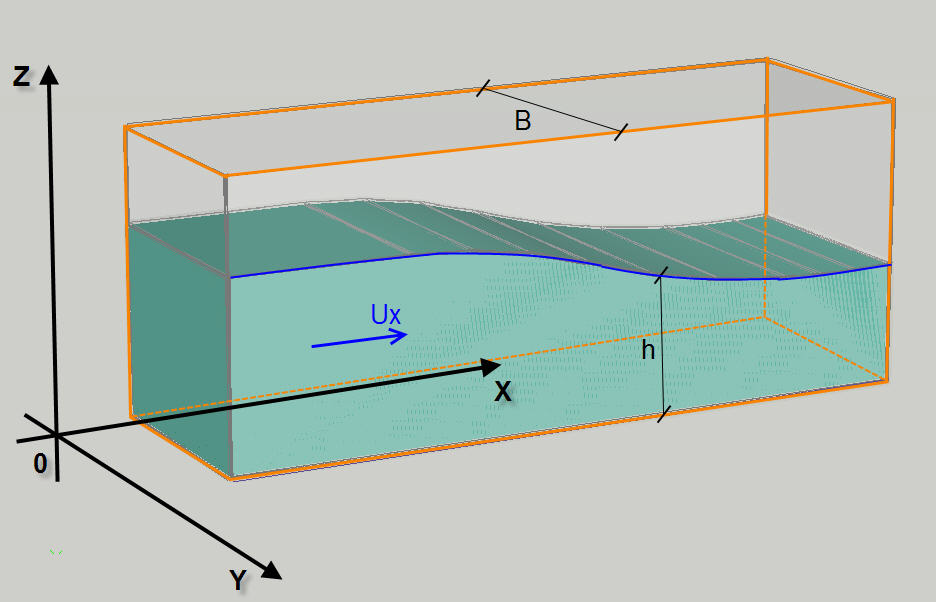
\includegraphics [scale = 0.5] {image1}
  \caption{К выводу уравнения движения.}
  \label{image1}
\end{figure}

Поскольку движение жидкости плавно изменяющееся живые сечения можно считать плоскими, а распределение давления в этих сечениях принять гидростатическим.
Таким образом, для величины давления в каждой точке такого потока должны выполняться уравнения равновесия покоящейся жидкости:

\begin{equation}
\left\{
  \label{eq_EulerStat}
{\setlength\arraycolsep{2pt}
  \begin{array}{rl}
     \vspace{5pt}
     \displaystyle X - \frac{1}{\rho} \frac{ \partial p}{ \partial x} = & 0  \\
     \vspace{5pt}
     \displaystyle Y - \frac{1}{\rho} \frac{ \partial p}{ \partial y} = & 0  \\
     \displaystyle Z - \frac{1}{\rho} \frac{ \partial p}{ \partial z} = & 0 \ ,
  \end{array}
}
\right.
\end{equation}

\noindent где $X,\ Y,\ Z$ -- проекции единичных массовых сил, действующих на рассматриваемую жидкость; 

$\rho$ -- плотность рассматриваемой жидкости; 

$p$ -- давление. \\

Так как давление распределено статически, величина давления в любом сечении потока зависит только от глубины (\ref{eq_p1}, \ref{eq_p2}), то при перемещении вдоль оси OX рассматриваемого потока давление будет изменяться со скоростью, зависящей только от приращения глубин. Определим величину этой скорости изменения давления, для этого рассмотрим поток жидкости с положительным уклоном свободной поверхности (рис.\ref{image2}). 

\newpage

\begin{figure} [ht]
  \center
  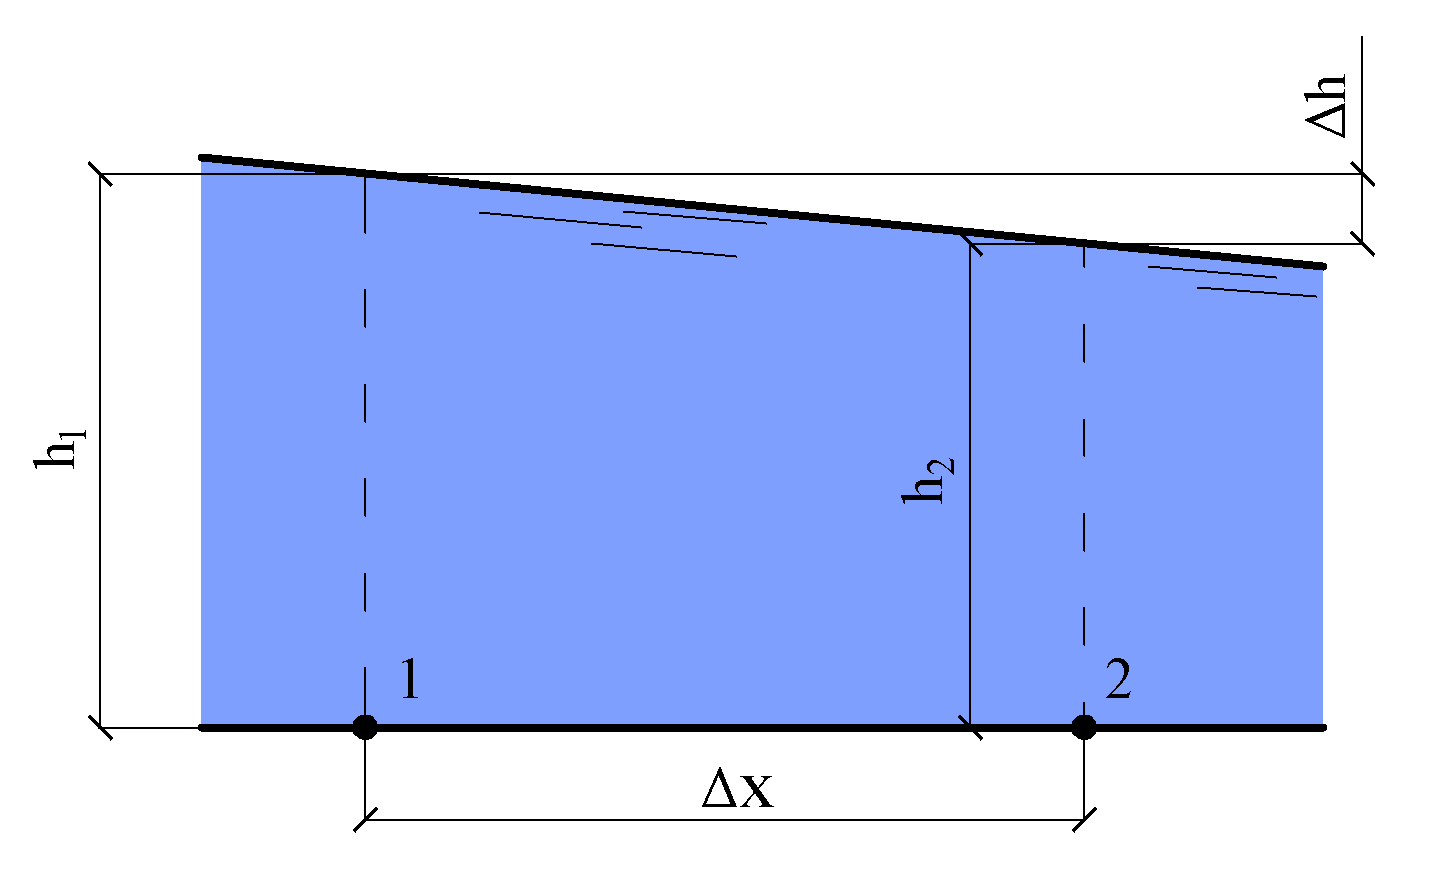
\includegraphics [scale = 0.8] {image2}
  \caption{К определению скорости изменения давления.}
  \label{image2}
\end{figure}

Поскольку давление в потоке распределено гидростатически, величина давления в точках 1 и 2 этого потока определяется по основному уравнению гидростатики:

\begin{equation}
  \label{eq_p1}
  p_1 = p_0 + \rho g h_1
\end{equation}

\begin{equation}
  \label{eq_p2}
  p_2 = p_0 + \rho g h_2
\end{equation}

При перемещении из точки 1 в точку 2, которые находятся на расстоянии $ \Delta x $ друг от друга, давление изменится на величину:

$$
  \Delta p = ( p_0 + \rho g h_2 ) - ( p_0 + \rho g h_1 ) = \rho g (h_2- h_1) = \rho g \Delta h \ ,
$$

\noindent где

$$
  \displaystyle \Delta h = h_2- h_1 = \frac{\partial h}{\partial x} \Delta x \ ,
$$

\noindent откуда

$$
  \displaystyle \Delta p = \rho g \frac{\partial h}{\partial x} \Delta x 
$$

И скорость изменения давления при перемещении вдоль оси OX:

\begin{equation}
  \label{eq_deltap_po_x}
  \displaystyle \frac{\partial p}{\partial x} = \frac{\Delta p} {\Delta x} = \rho g \frac{\partial h}{\partial x} \ ,
\end{equation}

\vspace{0.5cm}

Теперь запишем для рассматриваемого потока (рис.\ref{image1}) уравнения движения.

\begin{equation}
\left\{
  \label{eq_EulerDyn}
{\setlength\arraycolsep{2pt}
  \begin{array}{rl}
     \vspace{5pt}
     \displaystyle X' - \frac{1}{\rho} \frac{ \partial p}{ \partial x} - \frac{d U_x}{d t} = & 0  \\
     \vspace{5pt}
     \displaystyle Y' - \frac{1}{\rho} \frac{ \partial p}{ \partial y} - \frac{d U_y}{d t} = & 0  \\
     \displaystyle Z' - \frac{1}{\rho} \frac{ \partial p}{ \partial z} - \frac{d U_z}{d t} = & 0 \ ,
  \end{array}
}
\right.
\end{equation}

\noindent где $X', Y', Z'$ -- проекции единичных массовых сил, действующих в движущейся жидкости, причём:

\vspace{0.2cm}

$ \displaystyle X' = \frac{ -F_{friction} }{g} \neq X $, поскольку силы трения $ F_{friction} $ проявляются только в движении; 

$ Y' = 0 $;

$ Z' = Z = -g $. \\ 


В связи с тем, что для этого потока также справедлива система (\ref{eq_EulerStat}) то, так как $ Z = Z' $:

$$ 
  \displaystyle Z' - \frac{1}{\rho} \frac{\partial p}{\partial z} = 0
$$

После подстановки этого условия статического распределения давления в систему (\ref{eq_EulerDyn}) её третье уравнение (проекция на OZ) будет иметь вид:

$$
  \displaystyle \frac{d U_z}{d t} = 0
$$

Для перехода к двумерной задаче положим координату $ y = 0 $, исключив из рассмотрения второе уравнение системы (\ref{eq_EulerDyn}), при этом подразумевая, что ширина потока вовсе не нулевая, однако параметры, характеризующие состояние потока в этом направлении постоянны для каждого момента времени:

\begin{equation}
   \label{eq_uslov2d}
   \displaystyle \frac{\partial p}{\partial y} = 0 ;\  \frac{\partial U_x}{\partial y} = 0 ;\  \frac{\partial U_y}{\partial y} = 0 ;\  \frac{\partial U_z}{\partial y} = 0 .
\end{equation}

И, соответственно, система уравнений (\ref{eq_EulerDyn}) примет вид:

$$
   \left\{
{\setlength\arraycolsep{2pt}
  \begin{array}{rl}
     \vspace{5pt}
    & \displaystyle  X' - \frac{1}{\rho} \frac{ \partial p}{ \partial x} - \frac{d U_x}{d t} = 0  \\
    & \displaystyle  \frac{d U_z}{d t} = 0 
  \end{array}
}
\right.
$$

\vspace{1cm}

Рассмотрим первое уравнение получившейся системы:

\begin{equation}
  \label{eq_uravnDvi1}
  \displaystyle \frac{1}{\rho} \frac{ \partial p}{ \partial x} + \frac{d U_x}{d t} - X' = 0 \ ,
\end{equation}

\noindent где $ X' = -\frac{ F_{friction} }{g} $, $  \frac{\partial p}{\partial p} = \rho g \frac{\partial h}{\partial x} $ в соответствии с (\ref{eq_deltap_po_x}), а $ \frac{d U_x}{d t} $ является субстанциональной производной:

$$
  \displaystyle \frac{d U_x}{d t} = \frac{\partial U_x}{\partial t} + \frac{\partial U_x}{\partial x} U_x + \frac{\partial U_x}{\partial y} U_y + \frac{\partial U_x}{\partial z} U_z
$$

Из выражения (\ref{eq_uslov2d}) $ \frac{\partial U_x}{\partial y} = 0 $. Величину проекции скорости в направлении ОХ примем постоянной и равной средней на вертикали скорости $ U_x = U $ ($ \frac{\partial U_x}{\partial z} = 0 $), и, таким образом, от двумерной задачи перейдём к одномерной. Тогда:

\begin{equation}
  \label{eq_substU}
  \displaystyle \frac{d U_x}{d t} = \frac{\partial U_x}{\partial t} + \frac{\partial U_x}{\partial x} U_x = \frac{\partial U}{\partial t} + \frac{\partial U}{\partial x} U 
\end{equation}

С учётом вышесказанного (\ref{eq_deltap_po_x}, \ref{eq_substU}) перепишем выражение (\ref{eq_uravnDvi1}).

$$
  \displaystyle \frac{1}{\rho} \left( \rho g \frac{ \partial h}{ \partial x} \right) + \frac{\partial U}{\partial t} + \frac{\partial U}{\partial x} U + \frac{F_{friction}}{\rho} = 0
$$

\begin{equation}
  \label{eq_uravnDvi2}
\displaystyle g \frac{ \partial h}{ \partial x} + \frac{\partial U}{\partial t} + U \frac{\partial U}{\partial x} + \frac{F_{friction}}{\rho} = 0
\end{equation}

\vspace{1cm}

Величина силы трения $ F_{friction} $ в последнем выражении может быть определена по формуле Шези:

$$
  U = C\sqrt{RI} \ ,
$$

\noindent где $ U $ -- средняя скорость в рассматриваемом сечении; 

$ R $ -- гидравлический радиус; 

$ C $ -- коэффициент Шези; 

$ I = \frac{h_f} {l} $ -- гидравлический уклон; 

$ h_f $ -- потери полного напора на участке потока длиной $ l $. \\

Поскольку потери напора по физическому смыслу представляют собой изменение полной удельной энергии потока, отнесённые к единице веса рассматриваемой жидкости, то, учитывая что изменение полной удельной энергии потока происходит только за счёт работы сил трения $ A = F_{friction} \cdot l $ (равномерное движение):

$$
  \displaystyle h_f = \frac{F_{friction} \cdot l}{G} \ ,
$$

\noindent где $ G = \rho g 1 $ -- вес единичного объёма рассматриваемой жидкости. \\

Итак, уравнение Шези:

$$
  \displaystyle U = C \sqrt{R \frac{F_{friction} \cdot l}{l \rho g} }
$$

Откуда:

\begin{equation}
  \label{eq_Ffric}
  \displaystyle F_{friction} = \frac{U^2}{C^2 R} \cdot \rho g
\end{equation}

После подстановки полученного выражения для $ F_{friction} $ в выражение (\ref{eq_uravnDvi2}) получим окончательный вид уравнения движения мелкой воды.

\begin{equation}
  \label{eq_uravnDvi}
\displaystyle \frac{\partial U}{\partial t} + U \frac{\partial U}{\partial x} + g \frac{ \partial h}{ \partial x} + g \frac{U^2}{C^2 R} = 0
\end{equation}

\vspace{0.5cm}

Для того чтобы описать движение потока воды в одномерной постановке, уравнения (\ref{eq_uravnDvi}) недостаточно, необходимо дополнить его уравнением неразрывности.

\newpage

%--------------------------------------------------------------------------------------------------------------------
% вывод уравнения неразрывности
%--------------------------------------------------------------------------------------------------------------------

\subsection {Вывод уравнения неразрывности.}

Для вывода уравнения неразрывности рассмотрим неподвижный прямоугольный параллелепипед, сквозь который протекает поток жидкости.

\begin{figure} [ht]
  \center
  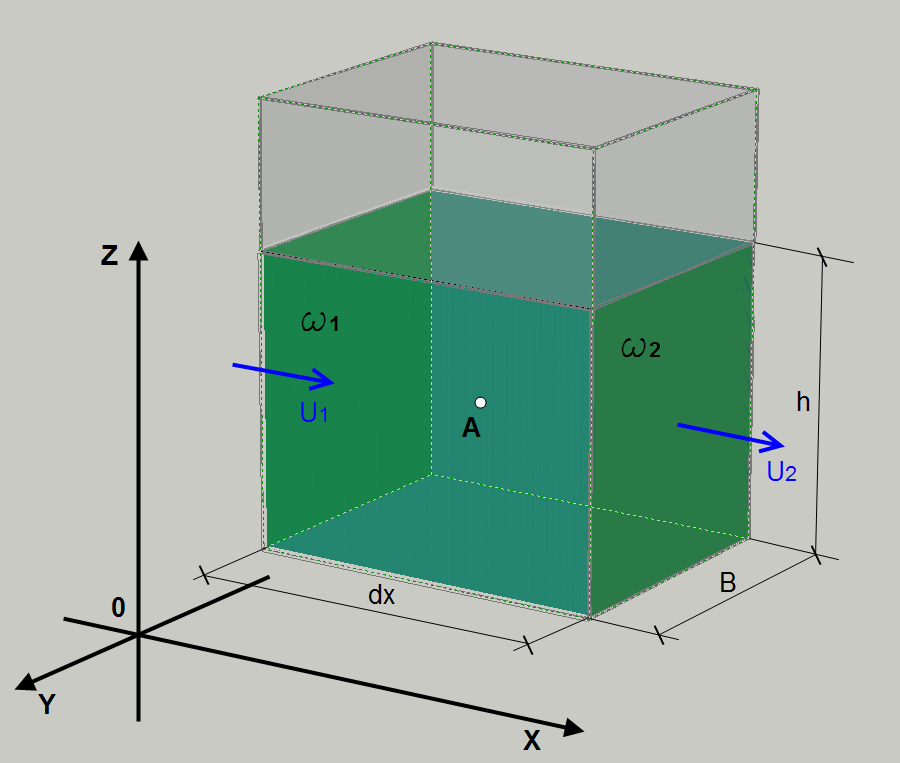
\includegraphics [scale = 0.4] {image3}
  \caption{К выводу уравнения неразрывности.}
  \label{img_image3}
\end{figure}

Рассматриваемый параллелепипед имеет длину $ d x $ вдоль потока жидкости, ширину $ B $ поперёк потока.

Поток жидкости движется вдоль оси OX. Скорости потока в пределах поперечных сечений $ \omega_1 $ и $ \omega_2 $ принимаются постоянными (средние скорости).

Предположим, что в течение некоторого промежутка времени расход потока жидкости неравномерно распределён вдоль оси OX. Такое предположение можно представить при условии, что поверхность жидкости в пределах параллелепипеда повышается вдоль оси ОХ\footnote{На самом деле поверхность в пределах параллелепипеда всегда параллельна плоскости XY, предположение о её уклоне вводится лишь для установки логической связи между изменением расхода вдоль ОХ и положением уровня жидкости.} (т.е. в сечении $ \omega_2 $ находится гребень продольной волны потока жидкости). В течение рассматриваемого промежутка времени вследствие действия сил тяжести поверхность жидкости будет стремиться к горизонтальной, а следовательно, расход жидкости, проходящий через сечение $ \omega_2 $ будет больше, чем расход через сечение $ \omega_1 $.

При таком изменении расхода (увеличении его вдоль ОХ) поверхность жидкости в параллелепипеде будет понижаться, причём вследствие малости величины $ dx $ можно считать, что положение свободной поверхности жидкости в параллелепипеде во всех точках (в плоскости XY) за промежуток времени $ dt $ изменится на одинаковую величину $ dh $.

Итак, за промежуток времени $ dt $ объём жидкости в параллелепипеде изменится. Поскольку уровень воды уменьшается со скоростью $ - \frac{dh}{dt} $, то приращение объёма параллелепипеда:

\begin{equation}
  \label{dvhparall}
  \displaystyle dV_h = -\frac{\partial h}{\partial t} dt B dx
\end{equation}

Это приращение объёма происходит за счёт того, что расход жидкости, поступающей в параллелепипед через сечение $ \omega_1 $ не равен расходу жидкости, выходящей из параллелепипеда через сечение $ \omega_2 $. То есть можно написать также:

$$
  dV_Q = \delta Q \cdot dt = (Q_2 - Q_1) dt
$$

Если предположить, что расход в центре параллелепипеда (в точке А) равен $ Q_A $ тогда расход, проходящий через сечение $ \omega_1 $:

$$
  \displaystyle Q_1 = Q_A - \frac{\partial Q}{\partial x} \frac{dx}{2} = Q_A - \frac{\partial (\omega U)}{\partial x} \frac{dx}{2}
$$

Расход, проходящий через сечение $ \omega_2 $:

$$
  \displaystyle Q_2 = Q_A + \frac{\partial Q}{\partial x} \frac{dx}{2} = Q_A + \frac{\partial (\omega U)}{\partial x} \frac{dx}{2}
$$

Тогда приращение объёма жидкости в параллелепипеде, обусловленное неравномерностью расхода вдоль ОХ:


$$
  \displaystyle dV_Q = \frac{\partial (\omega U)}{\partial x} dx dt
$$

Учитывая, что $ \omega = B \cdot h $, а также применяя правило дифференцирования произведения двух функций ($ h = f(x) $ и $ U = f(x) $) можно написать\footnote{Ширину потока $ B $ считаем постоянной величиной.}:

$$
  \displaystyle dV_Q = \frac{\partial (h \cdot U)}{\partial x} B \cdot dx dt
$$

$$
  \displaystyle dV_Q = \left( U \frac{\partial h}{\partial x} + h \frac{\partial U}{\partial x} \right)   B \cdot dx dt
$$


Поскольку $ dV_h = dV_Q $,

$$
  \displaystyle -\frac{\partial h}{\partial t} dt B dx = \left( U \frac{\partial h}{\partial x} + h \frac{\partial U}{\partial x} \right)   B \cdot dx dt
$$ 


И уравнение неразрывности в одномерной постановке задачи примет вид:

\begin{equation}
  \label{eq_urNerazr}
  \displaystyle \frac{\partial h}{\partial t} + U \frac{\partial h}{\partial x} + h \frac{\partial U}{\partial x} = 0
\end{equation}

\vspace{1.5cm}

Итак, система одномерных уравнений, позволяющих описать движение потока жидкости имеет вид:

\begin{equation}
  \label{eq_urMelk}
     \left\{
{\setlength\arraycolsep{2pt}
  \begin{array}{rl}
     \vspace{7pt}
    & \displaystyle \frac{\partial U}{\partial t} + U \frac{\partial U}{\partial x} + g \frac{ \partial h}{ \partial x} + g \frac{U^2}{C^2 R} = 0  \\
    & \displaystyle \frac{\partial h}{\partial t} + U \frac{\partial h}{\partial x} + h \frac{\partial U}{\partial x} = 0
  \end{array}
}
\right. 
\end{equation}

\newpage

%--------------------------------------------------------------------------------------------------------------------
% Решение системы
%--------------------------------------------------------------------------------------------------------------------


\section {Решение системы одномерных уравнений мелкой воды методом конечных разностей.}

\subsection{Метод конечных разностей.}

Решением системы уравнений при известных граничных условиях будет является функция, или несколько функций (по числу неизвестных параметров, входящих в систему уравнений), которые удовлетворяют решаемым уравнениям. Если эти функции не удаётся найти интегрированием дифференциальных уравнений, применяют численные методы. Одним из численных методов является метод конечных разностей.

Метод конечных разностей основывается на предположении, что искомое решение дифференциального уравнения существует, но пока неизвестна форма этого решения (имеет ли график решения форму прямой, параболы, синусоиды, и т.д.). И поскольку форма графика решения заранее неизвестна, его представляют как совокупность прямых линий, проведённых между двумя точками, лежащими на графике предполагаемого решения. Большее количество точек позволяет более детально описать предполагаемое решение. Уклон каждого отрезка, из которых состоит приближённое решение, представляет собой производную от функции предполагаемого решения в точке, находящейся где-то на части кривой предполагаемого решения, ограниченной точками рассматриваемого отрезка.

\begin{figure} [ht]
  \center
  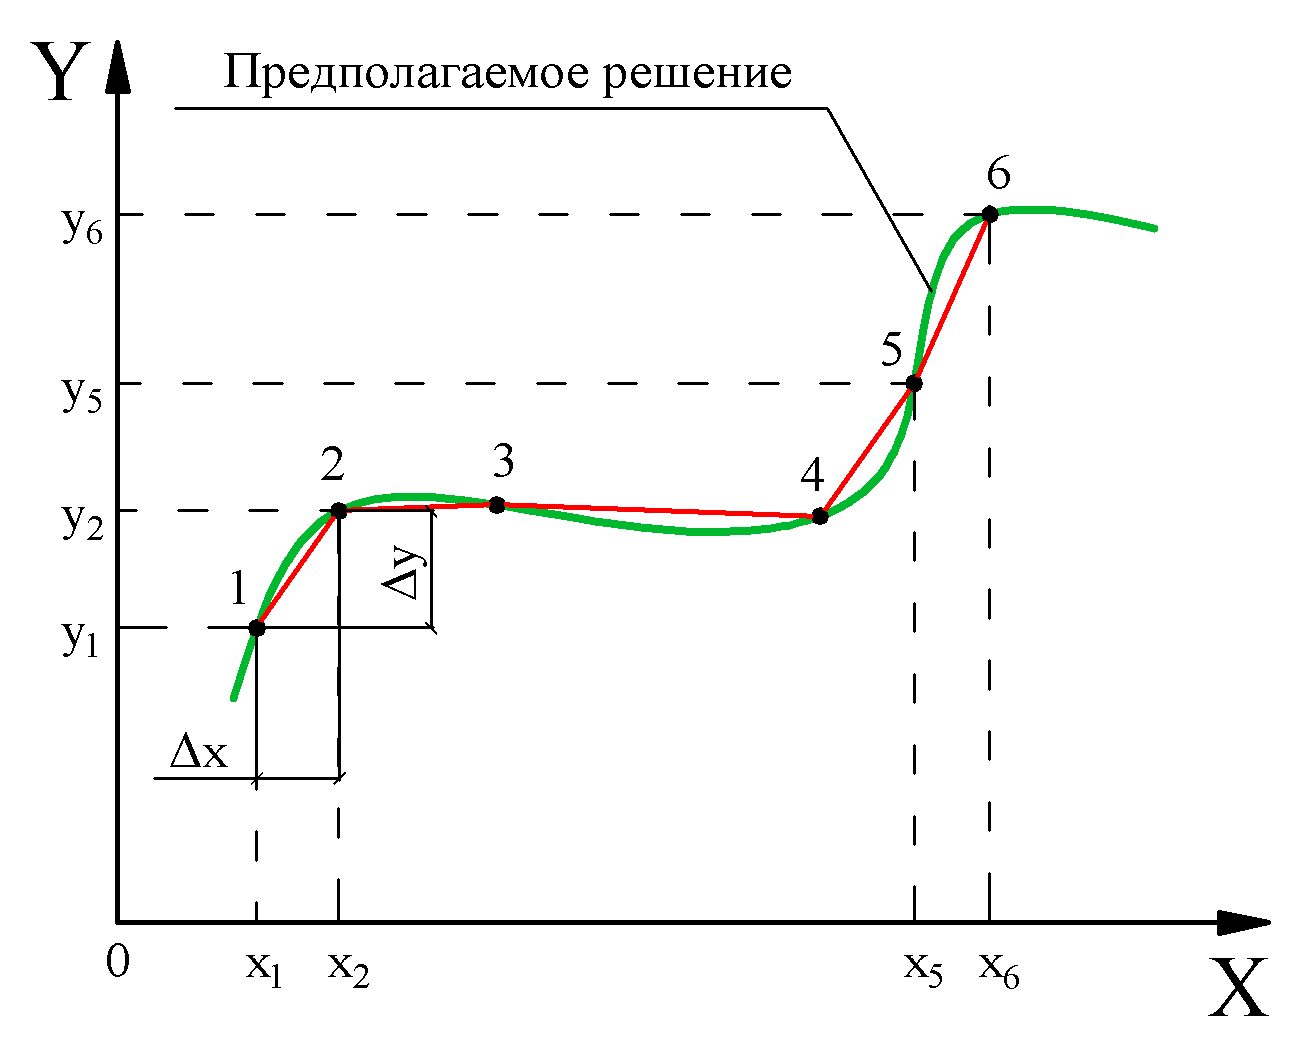
\includegraphics [scale = 0.9] {image4}
  \caption{Дискретизация дифференциального уравнения.}
  \label{img_image4}
\end{figure}

Так для отрезка 1-2 (рис.\ref{img_image4}):

$$
   \displaystyle \frac{\partial y}{\partial x} \approx \frac{\Delta y}{\Delta x} = \frac{y_2 - y_1}{x_2 - x_1} 
$$

Представленную таким образом производную можно подставить в решаемое уравнение, при этом становится возможным нахождения, например ординаты $ y_2 $ по заранее известным, или заданным величинам $ x_1 $, $ x_2 $ и $ y_1 $ и тогда найденный отрезок станет частью решения. Такую замену непрерывных производных их разностными аналогами называют дискретизацией.

Дискретизация дифференциальных уравнений может выполняться по различному количеству точек для представления производных, да и само представление производных может быть различным, то есть для решения дифференциальных уравнений могут применяться различные схемы дискретизации, обладающие различными свойствами.

Можно взглянуть на процесс дискретизации следующим образом: дифференциальное уравнение само по себе справедливо лишь для бесконечно малого участка пространства (точки). После дискретизации это уравнение оказывается справедливым для некоторого конечного объёма пространства, заключённого между точками, но с некоторым приближением. При этом оказывается важным, чтобы качество приближения было достаточным для того, чтобы полученное решение было близко к аналитическому решению, а не удалялось бы от него --- так проявляется свойство сходимости численной схемы.


%--------------------------------------------------------------------------------------------------------------------
% Дискретизация системы уравнений мелкой воды.
%--------------------------------------------------------------------------------------------------------------------


\subsection{Дискретизация системы уравнений мелкой воды.}

\subsubsection{Разностная сетка.}

В системе уравнений (\ref{eq_urMelk}), подлежащей решению искомыми функциями являются $ U $ и $ h $, которые могут изменяться во времени и вдоль координаты $ x $.

$$
  U = f(x,t) \ ;
$$

$$
  h = f(x,t) \ .
$$

Для определения точек дискретизации область пространства $ x, t $ разбивается $ n $ сечениями на $ n-1 $ интервалов вдоль оси ОХ и на $ m-1 $ временных слоёв с некоторым шагом по времени $ \tau $ .
  
\begin{figure} [ht]
  \center
  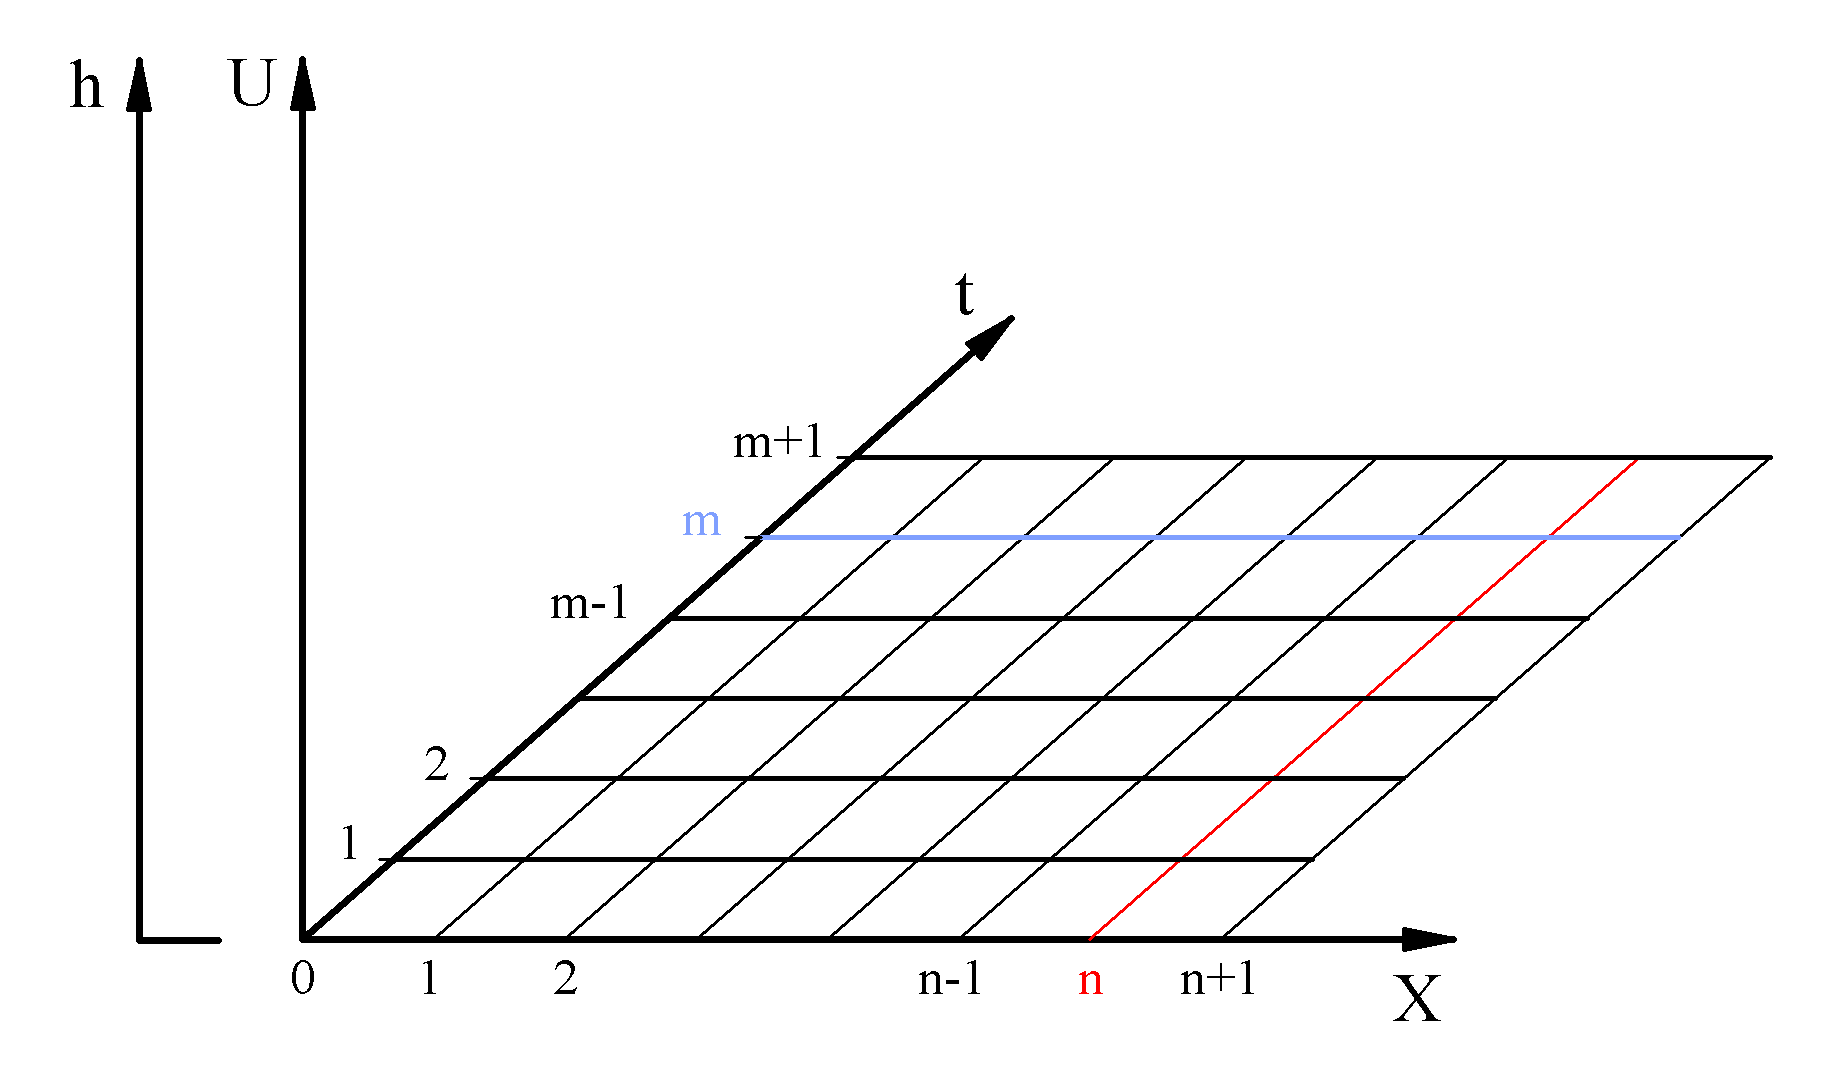
\includegraphics [scale = 0.9] {image5}
  \caption{Разностная сетка.}
  \label{img_image5}
\end{figure}

Для дискретизации системы уравнений (\ref{eq_urMelk}) будем использовать схему Прейсмана, согласно которой разностные аналоги производных вычисляются по выражениям:

\begin{equation}
   \label{eq_Preismann}
   \begin{array}{ll}
      \vspace{7pt}
      \displaystyle \frac{\partial U}{\partial t} = \frac{1}{2} \left( \frac{U_n^{m+1}- U_n^m}{\tau} + \frac{U_{n+1}^{m+1}- U_{n+1}^m}{\tau}\right)  \\
      \vspace{7pt}
      \displaystyle \frac{\partial U}{\partial x} = \theta \cdot \frac{U_{n+1}^{m+1} - U_n^{m+1}} {\Delta} + (1-\theta) \cdot \frac{U_{n+1}^m- U_n^m }{\Delta} \\
      \vspace{7pt}
      \displaystyle \frac{\partial h}{\partial t} = \frac{1}{2} \left( \frac{h_n^{m+1}- h_n^m}{\tau} + \frac{h_{n+1}^{m+1}- h_{n+1}^m}{\tau}\right)  \\
      \vspace{7pt}
      \displaystyle \frac{\partial h}{\partial x} = \theta \cdot \frac{h_{n+1}^{m+1} - h_n^{m+1}} {\Delta} + (1-\theta) \cdot \frac{h_{n+1}^m- h_n^m }{\Delta}
   \end{array} 
\end{equation}

\noindent где $ h_n^m, \ U_n^m $ -- значения глубины и скорости в точке с индексами $ n $ -- по оси ОХ и $ m $ -- по оси Ot;

$ \Delta $ -- расчётная длина интервала по оси ОХ; 

$ \tau $ -- расчётный промежуток времени; 

$ \theta $ -- Коэффициент схемы Прейсмана, принимающий значения от 0.5 до 1.0. \\


С помощью коэффициента $ \theta $ можно влиять на решение, получаемое для каждого слоя по времени. При $ \theta = 0.5 $ возмущения, создаваемые на предыдущем слое по времени в полной мере передаются расчётному (последующему) слою. При $ \theta > 0.5 $ такие возмущения со временем затухают. Под возмущением здесь можно иметь в виду отличные от нуля аналоги производных глубины или скорости потока в данной точке разностной сетки.

Схема Прейсмана является неявной --- это означает, что для расчётного промежутка времени известными величинами являются $ U_n^m $ и $ h_n^m $ скорости и глубины на предыдущем слое по времени, однако по этим значениям невозможно в явном виде вычислить значения $ U_n^{m+1} $ и $ h_n^{m+1} $ для этого приходится решать систему $ 2n - 2 $ (по числу расчётных интервалов вдоль оси ОХ) уравнений. Эту систему уравнений можно получить подстановкой значений (\ref{eq_Preismann}) для каждого расчётного интервала в систему (\ref{eq_urMelk}).

Поскольку значения $ U_n^m $ и $ h_n^m $ для предыдущего слоя по времени известны, то для удобства восприятия обозначим их заглавными буквами, а $ U_n^{m+1} $ и $ h_n^{m+1} $ расчётного слоя по времени обозначим прописными. В том случае, когда эти величины находятся в начале рассматриваемого интервала присвоим им индекс 1, в конце интервала --- индекс 2, то есть: \\

$ U_n^m $ -- обозначаем $ U_1 $ ;\\

$ U_{n+1}^m $ -- обозначаем $ U_2 $ ;\\

$ h_n^m $  -- обозначаем $ H_1 $ ;\\

$ h_{n+1}^m $  -- обозначаем $ H_2 $ ;\\

\noindent соответственно, для слоя по времени для которого составляется система уравнений:\\

 $ U_n^{m+1} $ -- $ u_1 $ ; \ \ \ \ \ $ U_{n+1}^{m+1} $ -- $ u_2 $ ;\\

$ h_n^{m+1} $ -- $ h_1 $ ; \ \ \ \ \ \ $ h_{n+1}^{m+1} $  -- $ h_2 $ .\\

\newpage

В итоге формулы для разностных аналогов производных по схеме Прейсмана примут вид:

\begin{equation}
   \label{eq_PreismannMod}
   \begin{array}{ll}
      \vspace{7pt}
      \displaystyle \frac{\partial U}{\partial t} = \frac{1}{2} \left( \frac{u_1- U_1}{\tau} + \frac{u_2- U_2}{\tau}\right)  \\
      \vspace{7pt}
      \displaystyle \frac{\partial U}{\partial x} = \theta \cdot \frac{u_2 - u_1} {\Delta} + (1-\theta) \cdot \frac{U_2- U_1 }{\Delta} \\
      \vspace{7pt}
      \displaystyle \frac{\partial h}{\partial t} = \frac{1}{2} \left( \frac{h_1- H_1}{\tau} + \frac{h_2- H_2}{\tau}\right)  \\
      \vspace{7pt}
      \displaystyle \frac{\partial h}{\partial x} = \theta \cdot \frac{h_2 - h_1} {\Delta} + (1-\theta) \cdot \frac{H_2 - H_1 }{\Delta}
   \end{array} 
\end{equation}

Поскольку в систему уравнений (\ref{eq_urMelk}) входят также значения $ U $ и $ h $, то при дискретизации заменим их соответствующими среднеарифметическими значениями, взятыми с предыдущего $ m $ слоя по времени:

\begin{equation}
   \label{eq_PreismannHiU}
   \begin{array}{ll}
      \vspace{7pt}
      \displaystyle U = \frac{U_1 + U_2}{2}  \\
      \vspace{7pt}
      \displaystyle h = \frac{H_1 + H_2}{2} 
   \end{array} 
\end{equation}


%--------------------------------------------------------------------------------------------------------------------
% Дискретизация уравнения движения.
%--------------------------------------------------------------------------------------------------------------------


\subsubsection{Дискретизация уравнения движения.}

Выполним дискретизацию уравнения движения для этого подставим выражения (\ref{eq_PreismannMod}, \ref{eq_PreismannHiU}) в первое уравнение системы (\ref{eq_urMelk}). В результате оно примет следующий вид:

$$
   \displaystyle \frac{1}{2} \left( \frac{u_1-U_1}{\tau} + \frac{u_2-U_2}{\tau} \right) + \frac{U_1+U_2}{2} \cdot \left[ \theta \frac{u_2 - u_1}{\Delta} + (1-\theta) \frac{U_2-U_1}{\Delta} \right] + \cdots   
$$

$$
   \displaystyle \cdots + g \cdot \left[ \theta \frac{h_2-h_1}{\Delta} + (1-\theta) \frac{H_2-H_1}{\Delta} \right] + \left( \frac{U_1+U_2}{2} \cdot \left| \frac{U_1+U_2}{2} \right| \right) \cdot \frac{g}{C^2R} = 0
$$

В последнем слагаемом в этом выражении величина $ \frac{U_1+U_2}{2} $ взята по модулю для того, чтобы учесть направление действия сил трения.

Теперь преобразуем это выражение, приведя его к виду линейного уравнения с коэффициентами при неизвестных ($ u_1, u_2, h_1, h_2 $) для расчётного слоя по времени.

$$
   \displaystyle U = \frac{U_1+U_2}{2}
$$


$$
   \displaystyle \frac{u_1-U_1}{2\tau} + \frac{u_2-U_2}{2\tau} + U \cdot \theta \frac{u_2-u_1}{\Delta} + U(1-\theta) \frac{U_2-U_1}{\Delta} + g \theta \frac{h_2-h_1}{\Delta} + \cdots
$$
$$
   \displaystyle \cdots + g(1-\theta) \frac{H_2-H_1}{\Delta} + \frac{g U |U|}{C^2 R} = 0
$$

\vspace{1cm}

$$
   \displaystyle \frac{u_1}{2\tau} - \frac{U_1}{2\tau} + \frac{u_2}{2\tau} - \frac{U_2}{2\tau} + \frac{U\theta u_2}{\Delta} - \frac{U\theta u_1}{\Delta} + \frac{U(1-\theta)(U_2-U_1)}{\Delta} + \frac{g\theta h_2}{\Delta} - \frac{g\theta h_1}{\Delta} + \cdots
$$
$$
   \displaystyle \cdots  + g(1-\theta) \frac{H_2-H_1}{\Delta} + \frac{g U |U|}{C^2 R}
    = 0
$$


\newpage

$$
   \displaystyle u_1 \left( \frac{1}{2\tau} - \frac{U\theta}{\Delta} \right) + u_2 \left( \frac{1}{2\tau} + \frac{U\theta}{\Delta} \right)  + h_1 \left( - \frac{g\theta}{\Delta} \right) +   h_2 \left( \frac{g\theta}{\Delta} \right) + \cdots
$$ 
$$
   \displaystyle \cdots + \left( \frac{1-\theta}{\Delta} \biggl[ U(U_2-U_1) + g(H_2-H_1) \biggr] - \frac{U_1+U_2}{2\tau} + \frac{g U |U|}{C^2 R} \right) = 0
$$

\vspace{1cm}

Теперь уравнение движения можно представить в виде:

\begin{equation}
\label{eq_urDviDiskr}
   \begin{array}{ll}
      \vspace{10pt}
                     u_1 \cdot a_1 + u_2 \cdot a_2 + h_1 \cdot b_1 + h_2 \cdot b_2 + K = 0 \ ,\textrm{в котором} \\
      \vspace{7pt}
      \displaystyle a_1 = \frac{1}{2\tau} - \frac{U\theta}{\Delta}  \ ;\\
      \vspace{7pt}
      \displaystyle a_2 = \frac{1}{2\tau} + \frac{U\theta}{\Delta}  \ ;\\
      \vspace{7pt}
      \displaystyle b_1 = - \frac{g\theta}{\Delta} \ ;\\
      \vspace{7pt}
      \displaystyle b_2 = \frac{g\theta}{\Delta} \ ;\\
      \vspace{7pt}
      \displaystyle K = \frac{1-\theta}{\Delta} \biggl[ U(U_2-U_1) + g(H_2-H_1) \biggr] - \frac{U_1+U_2}{2\tau} + \frac{g U |U|}{C^2 R}  \ ;\\
      \vspace{7pt}
      \displaystyle U = \frac{U_1+U_2}{2} \ .
   \end{array} 
\end{equation}



%--------------------------------------------------------------------------------------------------------------------
% Дискретизация уравнения неразрывности.
%--------------------------------------------------------------------------------------------------------------------


\subsubsection{Дискретизация уравнения неразрывности.}

Произведём дискретизацию уравнения неразрывности для этого выполним аналогичные действия со вторым уравнением системы (\ref{eq_urMelk}). Далее проиллюстрированы эти действия.

$$
   \displaystyle U = \frac{U_1+U_2}{2}
$$

$$
   \displaystyle H = \frac{H_1+H_2}{2}
$$

$$
   \displaystyle \frac{1}{2} \left( \frac{h_1-H_1}{\tau} + \frac{h_2-H_2}{\tau} \right) + U \cdot \left( \theta \frac{h_2-h_1}{\Delta} + (1-\theta) \frac{H_2-H_1}{\Delta} \right) + \cdots
$$
$$
   \displaystyle \cdots H \cdot \left( \theta \frac{u_2-u_1}{\Delta} + (1-\theta) \frac{U_2-U_1}{\Delta} \right) = 0
$$

\vspace{1cm}

$$
   \displaystyle \frac{h_1}{2\tau} - \frac{H_1}{2\tau} + \frac{h_2}{2\tau} - \frac{H_2}{2\tau} + \frac{U\theta h_2}{\Delta} -\frac{U\theta h_1}{\Delta} + \frac{U(1-\theta)(H_2-H_1)}{\Delta} + \frac{H\theta u_2}{\Delta}  \cdots
$$
$$
   \displaystyle \cdots -\frac{H\theta u_1}{\Delta} + \frac{H(1-\theta)(U_2-U_1)}{\Delta} = 0
$$

\vspace{1cm}

$$
   \displaystyle u_1 \left( - \frac{H\theta}{\Delta} \right) + u_2 \left( \frac{H\theta}{\Delta} \right) + h_1 \left( \frac{1}{2\tau} - \frac{U\theta}{\Delta} \right) + h_2 \left( \frac{1}{2\tau} + \frac{U\theta}{\Delta} \right) + \cdots
$$
$$
   \displaystyle \cdots + \left( \frac{1-\theta}{\Delta} \biggl[ U(H_2-H_1) + H(U_2-U_1) \biggr] - \frac{H_1+H_2}{2\tau} \right) = 0
$$

\vspace{1cm}

И, уравнения неразрывности в удобном для нас виде:

\begin{equation}
\label{eq_urNerDiskr}
   \begin{array}{ll}
      \vspace{10pt}
                     u_1 \cdot a_3 + u_2 \cdot a_4 + h_1 \cdot b_3 + h_2 \cdot b_4 + L = 0 \ ,\textrm{где} \\
      \vspace{7pt}
      \displaystyle a_3 = - \frac{H\theta}{\Delta}  \ ;\\
      \vspace{7pt}
      \displaystyle a_4 = \frac{H\theta}{\Delta}  \ ;\\
      \vspace{7pt}
      \displaystyle b_3 = \frac{1}{2\tau} - \frac{U\theta}{\Delta}  \ ;\\
      \vspace{7pt}
      \displaystyle b_4 = \frac{1}{2\tau} + \frac{U\theta}{\Delta} \ ;\\
      \vspace{7pt}
      \displaystyle L = \frac{1-\theta}{\Delta} \biggl[ U(H_2-H_1) + H(U_2-U_1) \biggr] - \frac{H_1+H_2}{2\tau} \ ;\\
      \vspace{7pt}
      \displaystyle U = \frac{U_1+U_2}{2} \ ;\\
      \vspace{7pt}
      \displaystyle H = \frac{H_1+H_2}{2} \ .
   \end{array} 
\end{equation}


%--------------------------------------------------------------------------------------------------------------------
% Постановка задачи.
%--------------------------------------------------------------------------------------------------------------------


\subsection[Постановка задачи.]{Постановка задачи моделирования процесса наполнения камеры судоходного шлюза с головной системой.}

Чтобы описать процесс наполнения камеры шлюза с головной системой питания будем использовать систему одномерных дифференциальных уравнений мелкой воды (\ref{eq_urMelk}).

Представим камеру судоходного шлюза в виде прямоугольного параллелепипеда, в котором на момент начала наполнения находится вода, заполняя его на глубину $ h_o $. Сам процесс наполнения будем представлять как поступление воды через одну из проницаемых торцевых стенок этого параллелепипеда с соответствующим изменением уровня воды. Количественная характеристика такого изменения уровня воды во времени может быть получена в результате решения системы уравнений мелкой воды, дополненной граничными условиями.

\begin{figure} [ht]
  \center
  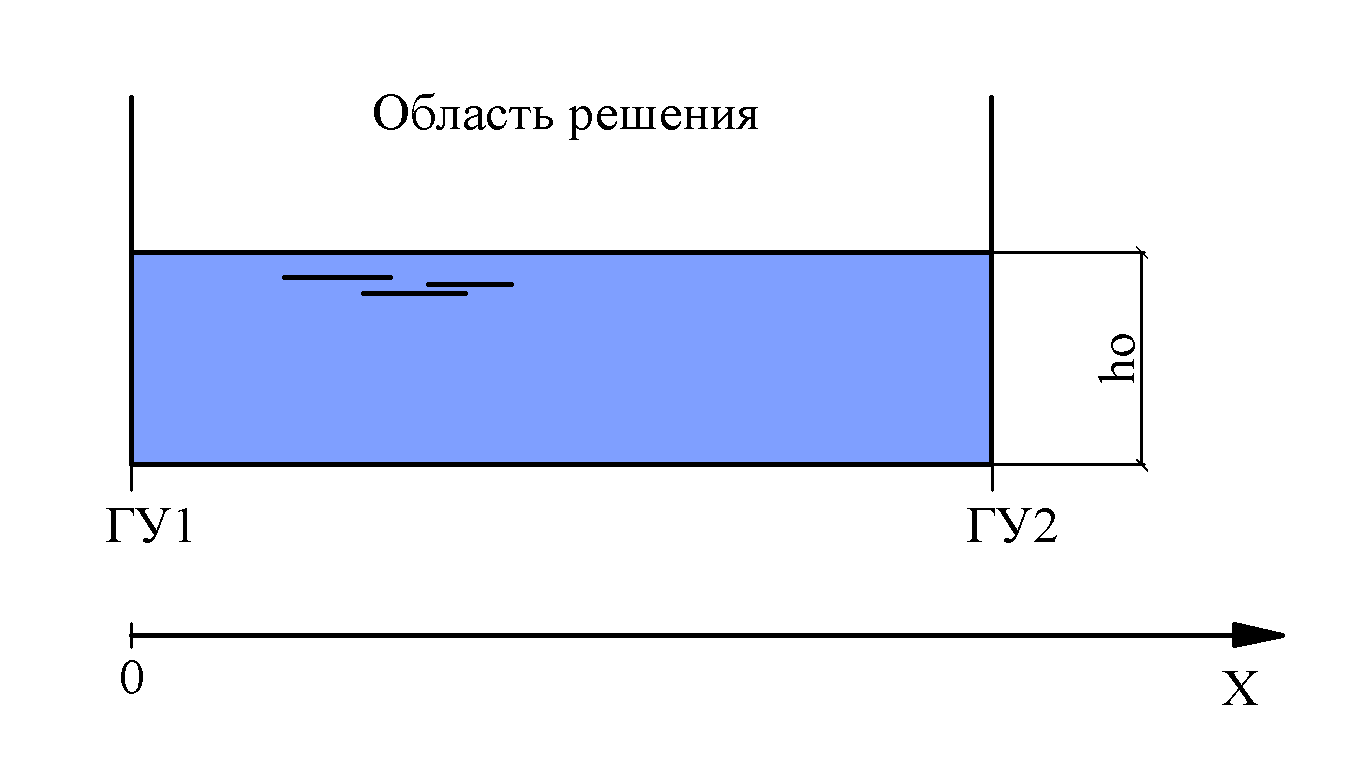
\includegraphics [scale = 0.9] {image6}
  \caption{Постановка задачи.}
  \label{img_image6}
\end{figure}

В качестве граничных условий будем задаваться известными значениями скоростей на торцах рассматриваемой камеры шлюза ГУ1 и ГУ2, причём на границе поступления расхода наполнения в камеру шлюза -- ГУ1, значение скорости может быть определено по зависимости:

$$
   \displaystyle \textrm{ГУ1:\ \ \ } u_{in} = \frac{Q}{BH},
$$

\noindent где $ Q $ -- значение расхода воды, поступающей в камеру в расчётный момент времени;

$ B $ -- ширина камеры шлюза;

$ H $ -- глубина воды в сечении поступления расхода \footnote{Принимается равной глубине на предыдущем слое по времени для упрощения процесса решения.}

На противоположном конце камеры шлюза, вследствие её непроницаемости, скорость потока должна равняться нулю.

$$
    \textrm{ГУ2:\ \ \ } u_{out} = 0
$$

Для применения к процессу наполнения судоходного шлюза уравнений мелкой воды в дискретной форме, камеру шлюза разбивают по длине на некоторое количество интервалов. Каждый такой интервал внутри области решения представляется значениями глубин $ h_1 $ и $ h_2 $ и скоростей $u_1$, $u_2$ на границах интервала. Эти значения связаны между собой системой уравнений (уравнения движения и уравнения неразрывности в дискретной форме):

\begin{equation}
\label{eq_urMelkDiskr}
   \left\{
   \begin{array}{ll}
      
      u_1 a_1 + u_2 a_2 + h_1 b_1 + h_2 b_2 + K = 0 \\
      u_1 a_3 + u_2 a_4 + h_1 b_3 + h_2 b_4 + L = 0
           
   \end{array}
   \right.
\end{equation}

\begin{figure} [ht]
  \center
  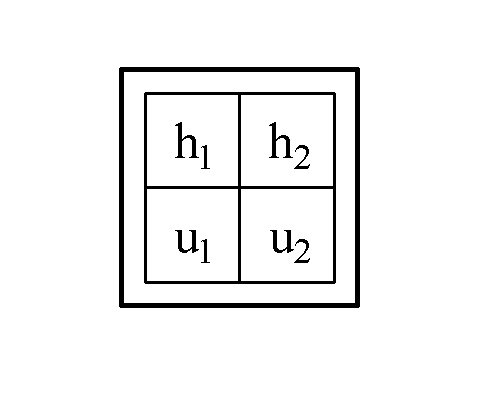
\includegraphics [scale = 0.9] {image7}
  \caption{Расчётный интервал.}
  \label{img_image7}
\end{figure}

 Для некоторого расчётного интервала $N$ примем обозначения:

$u_1^{<N>}$ -- значение скорости в начале интервала $N$;

$u_2^{<N>}$ -- значение скорости в конце интервала $N$;

$h_1^{<N>}$ -- значение глубины в начале интервала $N$;

$h_2^{<N>}$ -- значение глубины в конце интервала $N$;

\vspace{0.5cm}

Поскольку область решения в процессе дискретизации разбивается $n$ сечениями на $N = n-1$ интервалов, то для каждого последующего интервала значения $u_1$ и $h_1$ в его начале совпадают со значениями $u_2$ и $h_2$ в конце предыдущего интервала. Так, используя введённые обозначения можно написать:

\begin{equation}
\label{eq_intervKoop}
   u_2^{<N>} = u_1^{<N+1>}  \textrm{  и \ \ \ } h_2^{<N>} = h_1^{<N+1>}
\end{equation}

На основании этого, значения $u$ и $h$ в области решения для всех интервалов связаны между собой.

\begin{figure} [ht]
  \center
  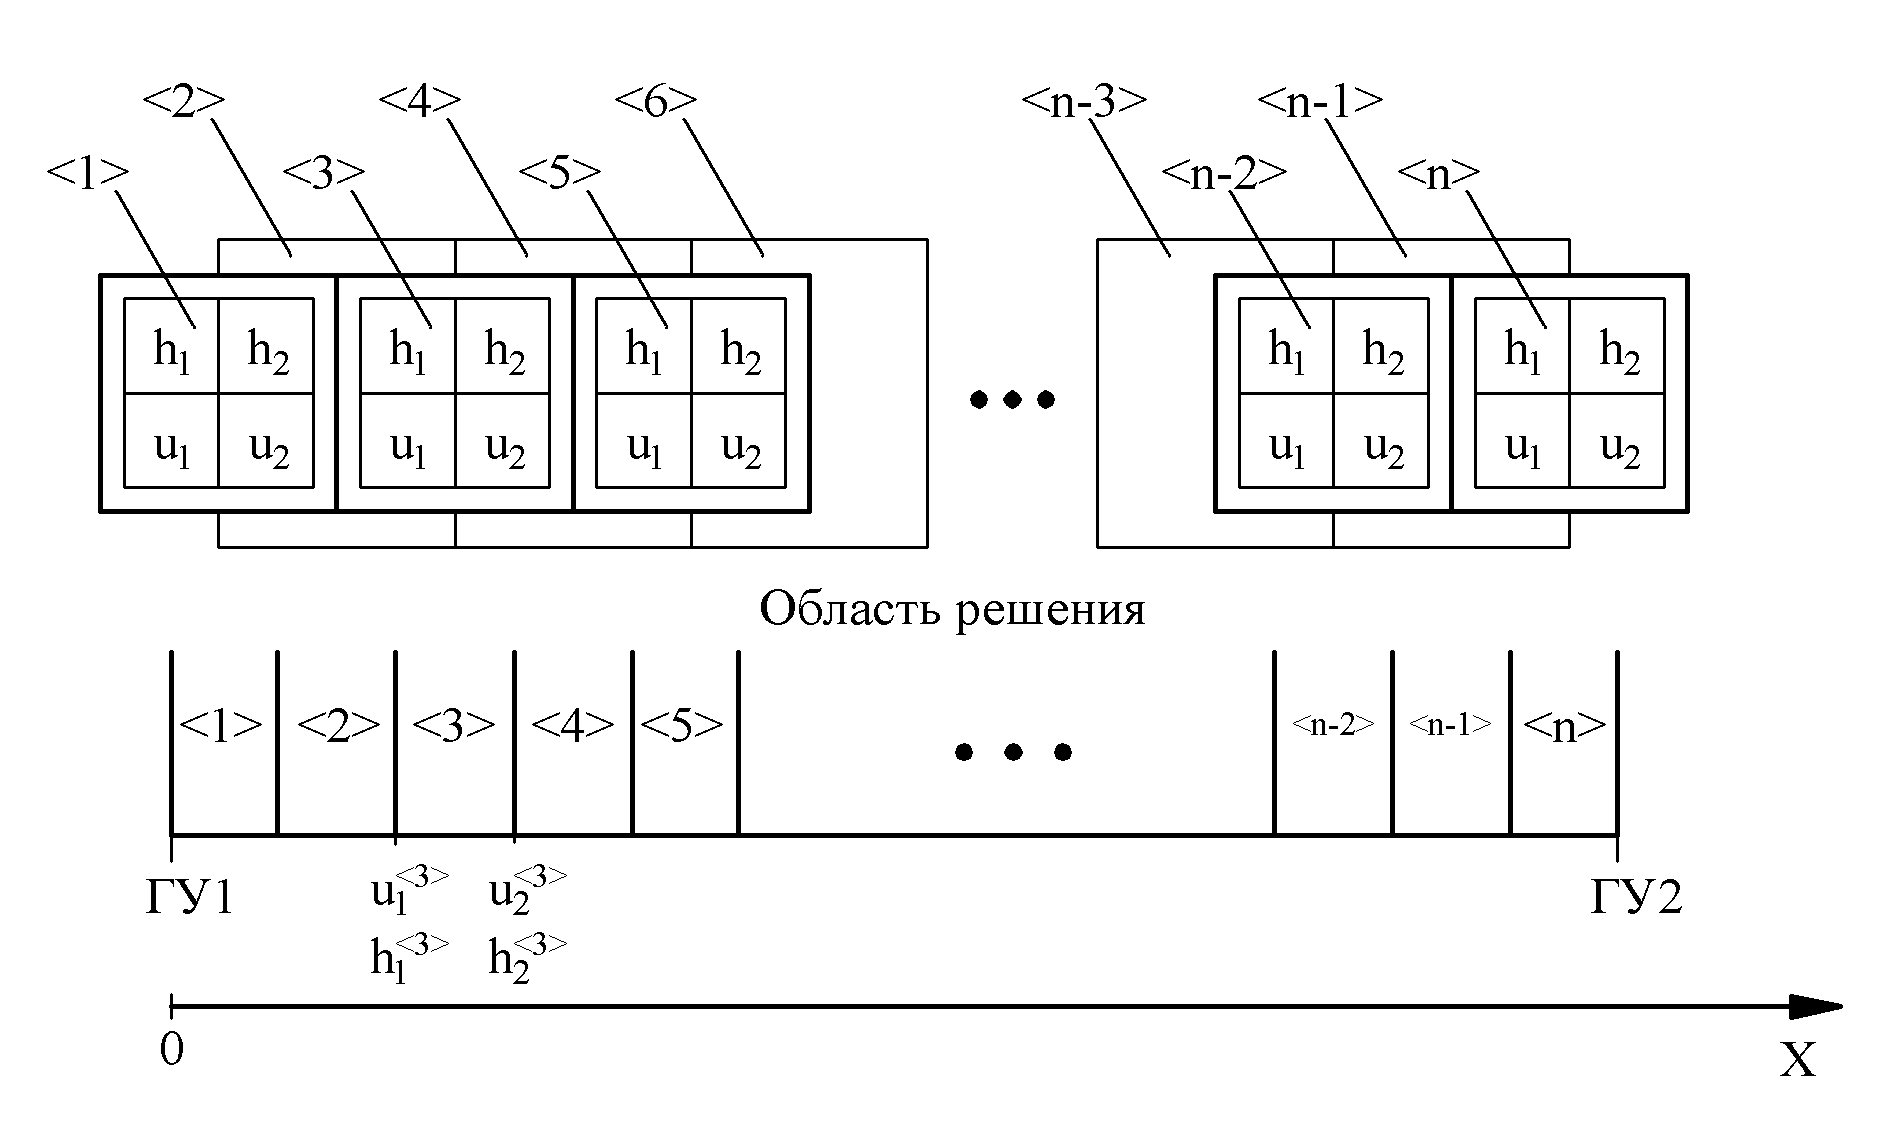
\includegraphics [scale = 0.9] {image8}
  \caption{Расчётные интервалы в области решения.}
  \label{img_image8}
\end{figure}

Таким образом, написав для каждого расчётного интервала систему уравнений мелкой воды в дискретной форме (\ref{eq_urMelkDiskr}) получаем систему уравнений для всей области решения, описывающую процесс наполнения камеры шлюза.

Особенными для получения решения являются: верхний граничный интервал $<1> $, в котором задано значение скорости $u_1^{<1>}$ и нижний граничный интервал $<N>$, в котором известна скорость $u_2^{<N>} = 0$.

\begin{equation}
\label{eq_urMelkDiskrAllKam}
   \left\{
   \begin{array}{ll}
      \vspace{0.5cm}
      \left.
      \begin{array}{ll}
      u_1^{<1>} a_1^{<1>} + u_2^{<1>} a_2^{<1>} + h_1^{<1>} b_1^{<1>} + h_2^{<1>} b_2^{<1>} + K^{<1>} &= 0 \\
      u_1^{<1>} a_3^{<1>} + u_2^{<1>} a_4^{<1>} + h_1^{<1>} b_3^{<1>} + h_2^{<1>} b_4^{<1>} + L^{<1>} &= 0
      \end{array}
      \right\} \textrm{Верх. гр.} \\
      
      \vspace{0.5cm}
      \left.
      \begin{array}{ll}
      u_1^{<2>} a_1^{<2>} + u_2^{<2>} a_2^{<2>} + h_1^{<2>} b_1^{<2>} + h_2^{<2>} b_2^{<2>} + K^{<2>} &= 0 \\
      u_1^{<2>} a_3^{<2>} + u_2^{<2>} a_4^{<2>} + h_1^{<2>} b_3^{<2>} + h_2^{<2>} b_4^{<2>} + L^{<2>} &= 0
      \end{array}
      \right\}  \textrm{Внутр. инт.} \\ 
      
      \vspace{0.2cm}
      \left.
      \begin{array}{ll}
      u_1^{<3>} a_1^{<3>} + u_2^{<3>} a_2^{<3>} + h_1^{<3>} b_1^{<3>} + h_2^{<3>} b_2^{<3>} + K^{<3>} &= 0 \\
      u_1^{<3>} a_3^{<3>} + u_2^{<3>} a_4^{<3>} + h_1^{<3>} b_3^{<3>} + h_2^{<3>} b_4^{<3>} + L^{<3>} &= 0
      \end{array}
      \right\}  \textrm{Внутр. инт.} \\ 
      
      \vspace{0.2cm}
      \hspace{5cm} \vdots \\
                 
      \left.
      \begin{array}{ll}
      u_1^{<N>} a_1^{<N>} + u_2^{<N>} a_2^{<N>} + h_1^{<N>} b_1^{<N>} + h_2^{<N>} b_2^{<N>} + K^{<N>} &= 0 \\
      u_1^{<N>} a_3^{<N>} + u_2^{<N>} a_4^{<N>} + h_1^{<N>} b_3^{<N>} + h_2^{<N>} b_4^{<N>} + L^{<N>} &= 0
      \end{array}
      \right\}  \textrm{Ниж. гр.} \\
           
   \end{array}
   \right.
\end{equation}

Эта система уравнений\footnote{Эту систему уравнений можно переписать с учётом (\ref{eq_intervKoop}) и, таким образом, уменьшить число неизвестных.} должна выполняться (поскольку мы считаем, что наполнение камеры описывается уравнениями мелкой воды) для всех интервалов в каждом расчётном $m+1$ слое по времени. Коэффициенты перед $u$ и $h$ определяются по соответствующим значениям глубины $H$ и скорости $U$ предыдущего слоя по времени.

Полученную систему уравнений можно решать различными методами. Далее предлагается решать её с помощью метода прогонки.



%--------------------------------------------------------------------------------------------------------------------
% Метод прогонки.
%--------------------------------------------------------------------------------------------------------------------


\subsubsection{Метод прогонки.}

Оставляя за рамками данной работы строгое математическое описание метода прогонки, рассмотрим реализацию этого метода применительно к системе уравнений (\ref{eq_urMelkDiskrAllKam}).

Метод прогонки состоит из двух последовательно выполняемых процедур: прямая прогонка и обратная прогонка.

Поскольку на верхнем граничном интервале в первом сечении задаётся граничное условие ГУ1, то есть известна величина скорости $u_1^{<1>}$, то остальные величины этого интервала ($h_1^{<1>}, h_2^{<1>}, u_2^{<1>}$) могут быть выражены через $u_1^{<1>}$ из уравнений (\ref{eq_urMelkDiskr}). Полученные выражения можно описать с помощью коэффициентов при неизвестных. Эти коэффициенты полностью описывают связь между неизвестными, хотя сами неизвестные ещё не определены (например, в уравнении прямой линии $Y = ax+b$, $a$ и $b$ -- коэффициенты уравнения). Таким образом, можно получить взаимосвязи между величинами $h$ и $u$ для всех интервалов в виде подобных коэффициентов.

Последовательно выражая неизвестные величины, входящие в систему уравнений (\ref{eq_urMelkDiskrAllKam}), начиная с уравнений для верхнего граничного интервала и заканчивая эту процедуру применительно у уравнениям для нижнего граничного интервала, окажется что все неизвестные величины выражены друг через друга. Полученные выражения для неизвестных описываются с помощью коэффициентов (типа $a$ и $b$ в примере с уравнением прямой).

Так как на нижнем граничном интервале задано граничное условие ГУ2, то последнее выражение для одной из неизвестных величин будет содержать лишь коэффициенты, а следовательно, значение этой неизвестной величины окажется найденным.

Таким образом, прямая прогонка -- это процедура нахождения коэффициентов для выражений всех неизвестных величин в системе (\ref{eq_urMelkDiskrAllKam}) друг через друга и определение одной из этих неизвестных величин на границе.

Далее выполняется обратная прогонка, заключающаяся в следующем: поскольку есть известные выражения, связывающие между собой все неизвестные величины (эти выражения ``сохраняются'' во время прямой прогонки в виде коэффициентов) то, так как одна из неизвестных величин на границе уже определена, то по имеющимся выражениям и этому известному значению вычисляются все остальные неизвестные величины.

\vspace{0.5cm}

Прямая прогонка.

Проиллюстрируем процесс получения зависимостей для коэффициентов, которые определяются в процедуре прямой прогонки. Для этого обратимся к системе уравнений (\ref{eq_urMelkDiskr}).

\begin{description}

\item[Шаг 1.] Из первого уравнения системы (\ref{eq_urMelkDiskr}) выразим $u_1$.
$$
   u_1 = f(h_1, h_2, u_2)
$$

\item[Шаг 2.] Из второго уравнения системы (\ref{eq_urMelkDiskr}) выразим $u_1'$.
$$
   u_1' = f(h_1, h_2, u_2)
$$

\item[Шаг 3.] Так как $u_1 = u_1'$,\ :
$$
   h_1 = f(h_2, u_2)
$$

\item[Шаг 4.] Из первого уравнения системы (\ref{eq_urMelkDiskr}) выразим $h_2$.
$$
   h_2 = f(h_1, u_1, u_2)
$$

\item[Шаг 5.] Из второго уравнения системы (\ref{eq_urMelkDiskr}) выразим $h_2'$.
$$
   h_2' = f(h_1, u_1, u_2)
$$

\item[Шаг 6.] Поскольку $u_1 = u_1'$, получим выражение для $u_2$\ :
$$
   u_2 = f(h_1, u_1)
$$

\end{description}

Полученные на шагах 3 и 6 выражения являются упрощением системы (\ref{eq_urMelkDiskr}), и поэтому справедливы для всех расчётных интервалов. Далее рассмотрим эти выражения отдельно для верхнего граничного интервала и всех остальных интервалов.

\vspace{0.5cm}

Верхний граничный интервал.

\begin{description}

\item[Шаг 7.] Поскольку значение $u_1$ известно, так как задано граничным условием, выражение полученное на шаге 6 преобразуется:
$$
  u_2 = f(h_1)
$$

\item[Шаг 8.] Подставив в это выражение выражение, полученное на шаге 3 мы получим:
$$
  u_2 = f(f(h_2, u_2)) 
$$
$$
  u_2 = f(h_2)
$$

\end{description}

\vspace{0.5cm}

Внутренние интервалы и нижний граничный интервал (для них нам также ``интересно''  получить выражения, связывающие $v_2$ и $h_2$).

\begin{description}

\item[Шаг 9.] В выражение, полученное на шаге 6, подставим выражение для $h_1$ с шага 3.
$$
  u_2 = f(f(h_2, u_2), u_1)
$$
$$
  u_2 = f(h_2, u_1)
$$

\item[Шаг 10.] Поскольку $u_1$ на данном интервале совпадает с $u_2^{<\textrm{пред.}>}$ на предыдущем интервале (см. Рис.\ref{img_image8}) и $h_1$ совпадает с $h_2^{<\textrm{пред.}>}$, подставим в выражение, полученное на 9 шаге, выражение для $u_1 = u_2^{<\textrm{пред.}>}$ с предыдущего интервала.
$$
  u_2 = f(h_2, u_2^{<\textrm{пред.}>})
$$
$$
  u_2 = f(h_2, f^{\textrm{<пред.>}}(h_2^{<\textrm{пред.}>}))
$$
$$
  u_2 = f(h_2, f^{\textrm{<пред.>}}(h_1)),\ \ \textrm{т.к. } h_2^{<\textrm{пред.}>} = h_1
$$

\item[Шаг 11.] В полученное выражение подставим выражение для $h_1$ с шага 3.
$$
  u_2 = f(h_2, f^{\textrm{<пред.>}}(f(h_2, u_2)))
$$
$$
  u_2 = f(h_2)
$$
\end{description}

И так для всех интервалов. В нижнем граничном интервале, в соответствии с ГУ2, известно значение $u_2$, поэтому по выражению с шага 11 можно найти $h_2$, что даёт возможность начать обратную прогонку.

Перед тем как привести формулы для процедуры обратной прогонки, рассмотрим более подробно шаги нахождения коэффициентов прямой прогонки.

\vspace{0.5cm}

\begin{description}

\item[Шаг 1:]
$$
  \displaystyle u_1 = \frac{-K - h_2 b_2 - h_1 b_1 - u_2 a_2}{a_1} 
$$

\item[Шаг 2:]
$$
  \displaystyle u_1' = \frac{-L - h_2 b_4 - h_1 b_3 - u_2 a_4}{a_3} 
$$

\item[Шаг 3:] $u_1 = u_1'$
$$
  \displaystyle \frac{-K - h_2 b_2 - h_1 b_1 - u_2 a_2}{a_1} = \frac{-L - h_2 b_4 - h_1 b_3 - u_2 a_4}{a_3} 
$$
$$
  \displaystyle K + h_2 b_2 + h_1 b_1 + u_2 a_2 = (L+h_2 b_4 + h_1 b_3 + u_2 a_4)\frac{a_1}{a_3}
$$
$$
  \displaystyle h_1 b_1 - \frac{h_1 b_3 a_1}{a_3} = (L+h_2 b_4 + u_2 a_4) \frac{a_1}{a_3} - (K+h_2 b_2 + u_2 a_2)
$$

$$
  \displaystyle h_1 = (L+ h_2 b_4 + u_2 a_4)W_1 - (K+h_2 b_2 + u_2 a_2)W_2\ \ ,\textrm{ где}
$$

$$
  \begin{array}{ll}
  \vspace{0.5cm}
  \displaystyle W_1 = \frac{a_1}{a_3 \left( b_1 - \displaystyle \frac{b_3 a_1}{a_3} \right)} \\
  \displaystyle W_2 = \frac{1}{ b_1 - \displaystyle \frac{b_3 a_1}{a_3}}
  \end{array}
$$

$$
  h_1 = u_2(a_4 W_1 - a_2W_2) + h_2(b_4W_1-b_2W_2) + (L \cdot W_1-K \cdot W_2)
$$

и, окончательно:

\begin{equation}
\label{eq_h1}
  \begin{array}{ll}
  \vspace{0.3cm}
  h_1 = u_2Q_1 + h_2Q_2 + Q_3 \ \ , \textrm{ где} \\
  \vspace{0.3cm}
  Q_1 = a_4W_1 - a_2W_2 \\
  \vspace{0.3cm}
  Q_2 = b_4W_1 - b_2W_2 \\
  \vspace{0.3cm}
  Q_3 = L \cdot W_1 - K \cdot W_2 \\
  \vspace{0.3cm}
  \displaystyle W_2 = \frac{1}{ b_1 - \displaystyle \frac{b_3 a_1}{a_3}} \\
  
  \displaystyle W_1 = W_2 \cdot \frac{a_1}{a_3} 
  
  \end{array}
\end{equation}

\vspace{0.5cm}

\item[Шаг 4:]
$$
  \displaystyle h_2 = \frac{-K - h_1 b_1 - u_2 a_2 - u_1 a_1}{b_2} 
$$

\item[Шаг 5:]
$$
  \displaystyle h_2' = \frac{-L - h_1 b_3 - u_2 a_4 - u_1 a_3}{b_4} 
$$

\item[Шаг 6:] $h_2 = h_2'$
$$
  \displaystyle \frac{-K - h_1 b_1 - u_2 a_2 - u_1 a_1}{b_2} = \frac{-L - h_1 b_3 - u_2 a_4 - u_1 a_3}{b_4} 
$$

$$
  \displaystyle K+ h_1b_1 + u_2a_2 + u_1a_1 = (L+h_1b_3 + u_2a_4 + u_1a_3) \frac{b_2}{b_4}
$$

$$
  \displaystyle u_2a_2 - u_2 \frac{a_4b_2}{b_4} = (L+h_1b_3+ u_1a_3) \frac{b_2}{b_4} - (K+h_1b_1 + u_1a_1)
$$

$$
  \displaystyle u_2 = (L + h_1b_3+u_1a_3)W_3 - (K+h_1b_1+u_1a_1)W_4 \ \ ,\textrm{ где}
$$

$$
  \begin{array}{ll}
  \vspace{0.5cm}
  \displaystyle W_3 = \frac{b_2}{b_4 \left( a_2 - \displaystyle \frac{a_4 b_2}{b_4} \right)} \\
  \displaystyle W_4 = \frac{1}{ a_2 - \displaystyle \frac{a_4 b_2}{b_4}}
  \end{array}
$$

$$
  u_2 = u_1(a_3W_3 - a_1W_4) + h_1(b_3W_3 - b_1W_4) + (L \cdot W_3 - K \cdot W_4)
$$

и, окончательно:

\begin{equation}
\label{eq_u2}
  \begin{array}{ll}
  \vspace{0.3cm}
  u_2 = u_1M_1 + h_1M_2 + M_3 \ \ , \textrm{ где} \\
  \vspace{0.3cm}
  M_1 = a_3W_3 - a_1W_4 \\
  \vspace{0.3cm}
  M_2 = b_3W_3 - b_1W_4 \\
  \vspace{0.3cm}
  M_3 = L \cdot W_3 - K \cdot W_4 \\
  \vspace{0.3cm}
  \displaystyle W_4 = \frac{1}{ a_2 - \displaystyle \frac{a_4 b_2}{b_4}} \\
  
  \displaystyle W_3 = W_4 \cdot \frac{b_2}{b_4} 
  
  \end{array}
\end{equation}

\vspace{0.5cm}

\item[Шаг 7:] $u_1 = u_{in}$
$$
  u_2 = u_{in} M_1 + h_1M_2 + M_3
$$

\item[Шаг 8:]
$$
  u_2 = u_{in}M_1 + (u_2Q_1+h_2Q_2+Q_3)M_2 + M_3 \ ,
$$

откуда

$$
  \displaystyle u_2 = h_2 \left( \frac{Q_2M_2}{1-Q_1 M_2} \right) + \frac{u_{in}M_1 + Q_3M_2 + M_3}{1- Q_1M_2}
$$

\begin{equation}
\label{eq_u2prFirst}
  \begin{array}{ll}
     \vspace{0.3cm}
     u_2 = h_2 K_1 + K_2 \ \ ,\textrm{ где} \\
     \vspace{0.3cm}
     \displaystyle K_1 = \frac{Q_2 M_2}{1-Q_1M_2}  \\
     \displaystyle K_2 = \frac{u_{in}M_1 +Q_3M_2 + M_3}{1-Q_1M_2}
  \end{array}
\end{equation}

\item[Шаг 9:]
$$
  u_2 = u_1M_1 + (u_2Q_1 + h_2Q_2 + Q_3)M_2 + M_3
$$

\item[Шаг 10:]
$$
  u_1 = u_2^{\textrm{<пр>}}  = K_1^{\textrm{<пр>}} h_2^{\textrm{<пр>}} + K_2^{\textrm{<пр>}}
$$

$$ \textrm{т.к. } h_2^{\textrm{<пр>}} = h_1 $$

$$
   u_1 = K_1^{\textrm{<пр>}} h_1 + K_2^{\textrm{<пр>}}
$$

$$
   u_2 = \left( K_1^{\textrm{<пр>}} h_1 + K_2^{\textrm{<пр>}} \right) M_1 + (u_2Q_1 + h_2Q_2 + Q_3)M_2 + M_3
$$

\item[Шаг 11:]
$$
   u_2 = \left( K_1^{\textrm{<пр>}} (u_2Q_1+h_2Q_2+Q_3) + K_2^{\textrm{<пр>}} \right) M_1 + (u_2Q_1 + h_2Q_2 + Q_3)M_2 + M_3
$$

$$
   u_2 - K_1^{\textrm{<пр>}}u_2Q_1M_1 - u_2Q_1M_2 = (h_2Q_2+Q_3)( K_1^{\textrm{<пр>}} M_1 + M_2) + K_2^{\textrm{<пр>}} M_1 + M_3
$$

$$
  u_2 = h_2 \frac{Q_2(K_1^{\textrm{<пр>}} M_1 + M_2)}{1-K_1^{\textrm{<пр>}}Q_1M_1 - Q_1M_2} + \frac{Q_3(K_1^{\textrm{<пр>}} M_1 +M_2) + K_2^{\textrm{<пр>}}M_1 + M_3 }{1-K_1^{\textrm{<пр>}}Q_1M_1 - Q_1M_2}
$$

\vspace{0.3cm}
и, окончательно:

\begin{equation}
\label{eq_u2prInner}
  \begin{array}{ll}
  \vspace{0.4cm}
  u_2 = h_2K_1 + K_2 \ \ , \textrm{ где} \\
  \vspace{0.4cm}
  \displaystyle K_1 = \frac{Q_2(K_1^{\textrm{<пр>}} M_1 + M_2)}{1-K_1^{\textrm{<пр>}}Q_1M_1 - Q_1M_2} \\
  \displaystyle K_2 = \frac{Q_3(K_1^{\textrm{<пр>}} M_1 +M_2) + K_2^{\textrm{<пр>}}M_1 + M_3 }{1-K_1^{\textrm{<пр>}}Q_1M_1 - Q_1M_2} \\ 
  
  \end{array}
\end{equation}

\end{description}

\vspace{0.3cm}

Обратная прогонка.

